\addcontentsline{toc}{chapter}{Appendices}

% The \appendix command resets the chapter counter, and changes the chapter numbering scheme to capital letters.
\appendix

\chapter{Supplementary Figures and Tables}
\label{appendixlabel1}

\begin{figure}[H]
\centering
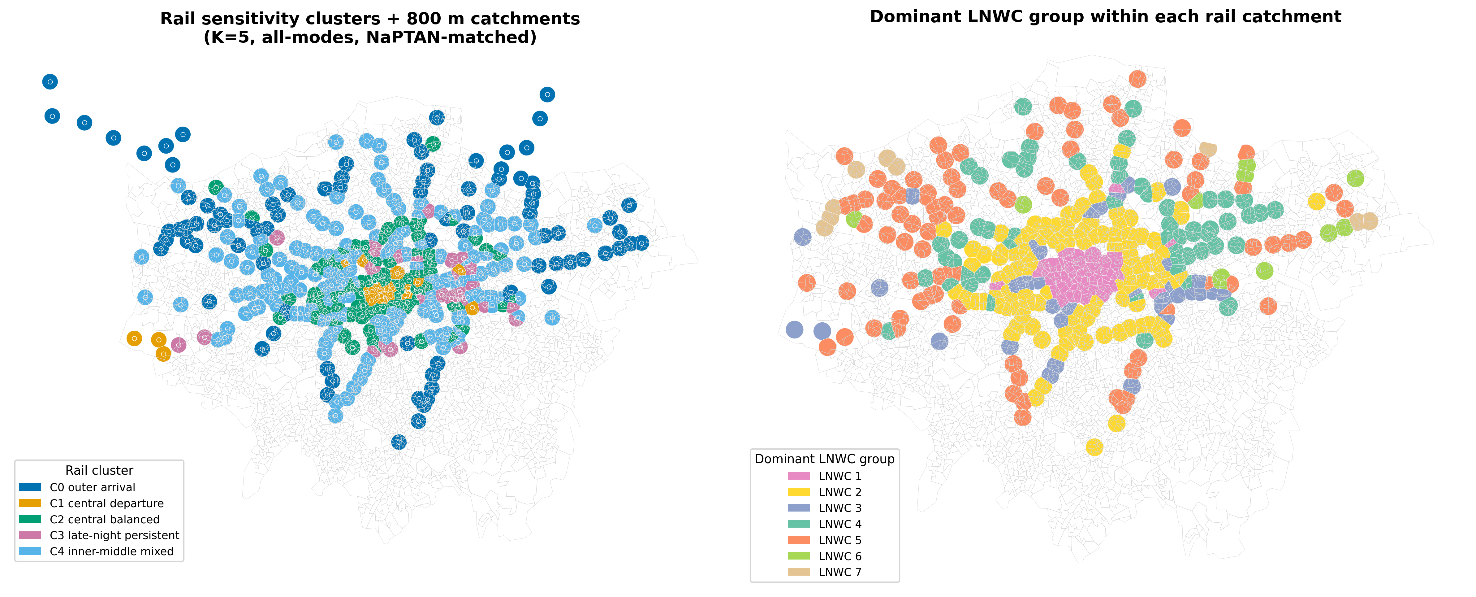
\includegraphics[width=\textwidth]{figures/appA_fig18.png}
\caption[Rail usage types and LNWC context]{Supplementary spatial comparison of Rail usage types and LNWC context within the mode-specific contextual-analysis samples}
\end{figure}

\begin{figure}[H]
\centering
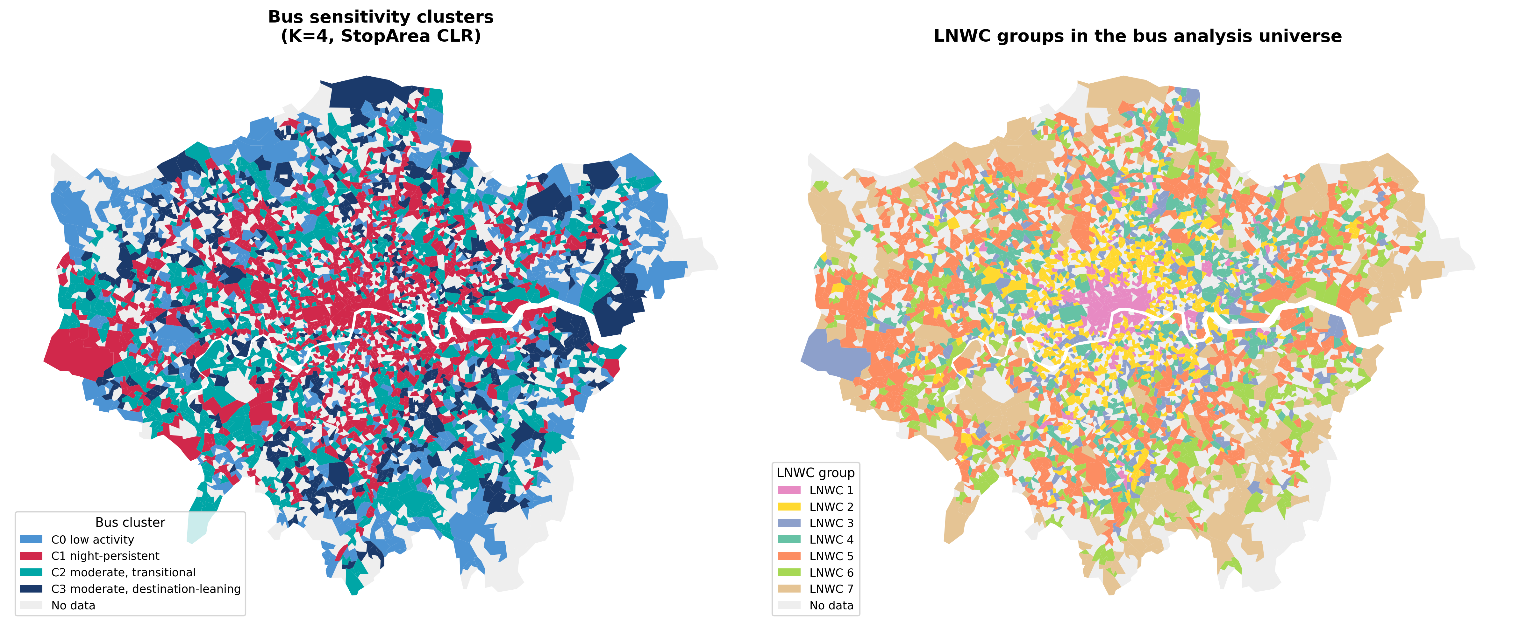
\includegraphics[width=\textwidth]{figures/appA_fig19.png}
\caption[Bus usage types and LNWC context]{Supplementary spatial comparison of Bus usage types and LNWC context within the mode-specific contextual-analysis samples}
\end{figure}

\begin{figure}[H]
\centering
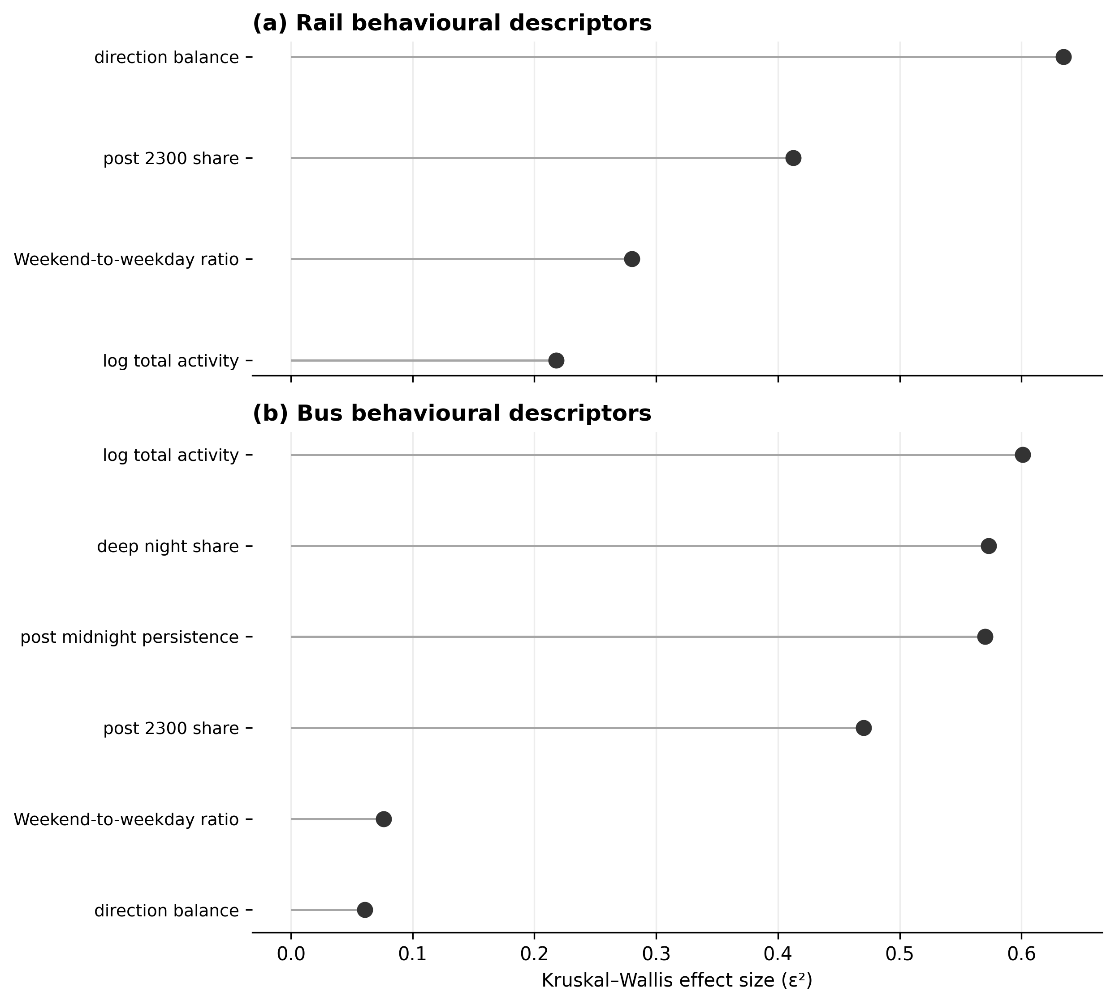
\includegraphics[width=0.85\textwidth]{figures/appA_fig20.png}
\caption[Behavioural-descriptor effect sizes]{Effect-size ranking of post-clustering behavioural descriptors across the Rail and Bus usage types: (a) Rail; (b) Bus.}
\end{figure}

\clearpage
\begin{figure}[H]
\centering
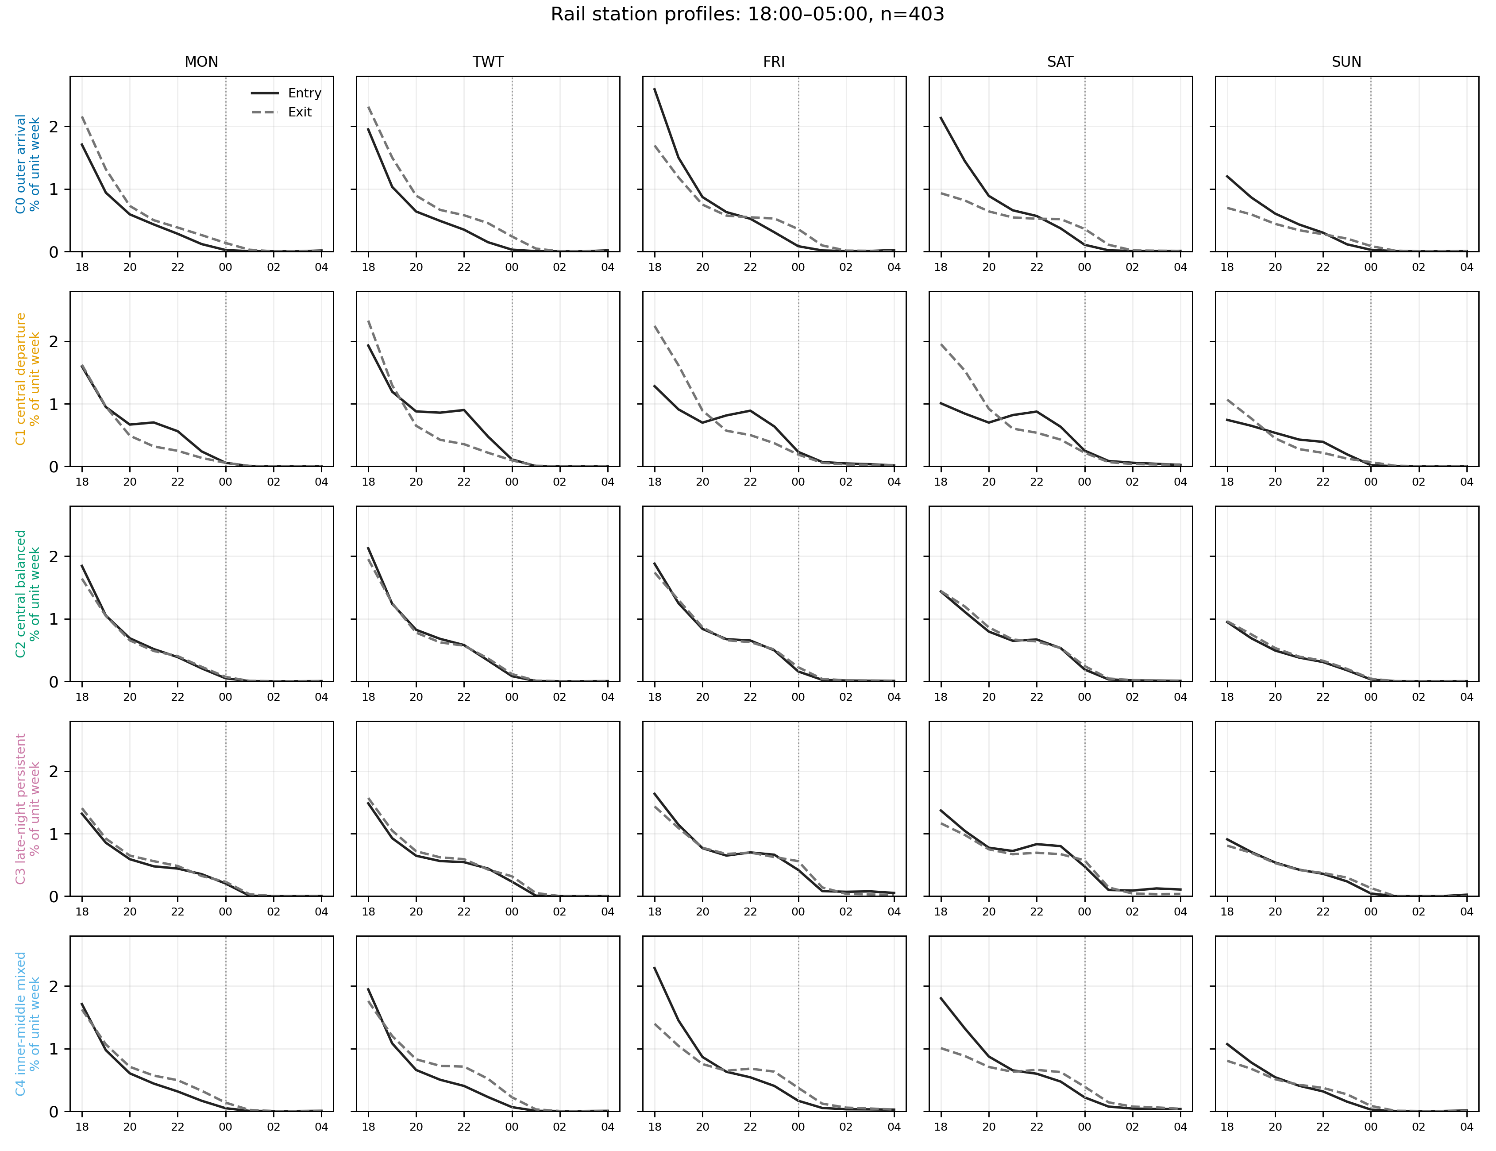
\includegraphics[width=\textwidth]{figures/appA_fig21.png}
\caption[Rail time-series feature map]{Original time-series feature map of Rail.}
\end{figure}

\clearpage
\begin{figure}[H]
\centering
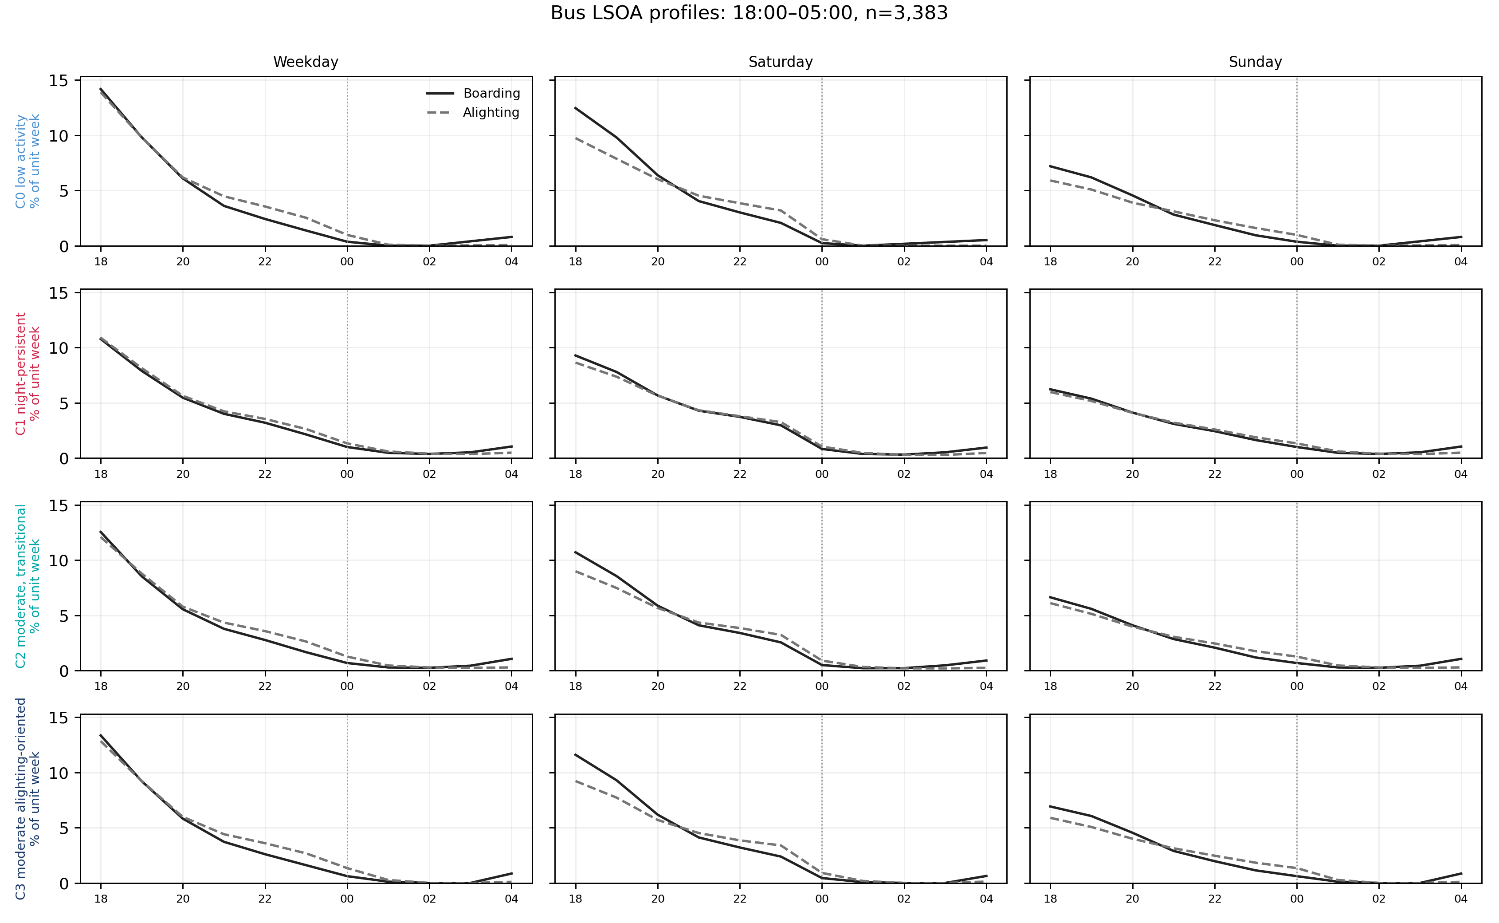
\includegraphics[width=\textwidth]{figures/appA_fig22.png}
\caption[Bus time-series feature map]{Original time-series feature map of the Bus.}
\end{figure}

\begin{landscape}
\begingroup
\small
\setlength{\tabcolsep}{5pt}
\renewcommand{\arraystretch}{1.12}
% AUTO-GENERATED from docx appendix data. Do not hand-edit numeric cells.

\small
\clearpage
\begin{longtable}{@{}p{4.2cm} r r r r r r@{}}
\caption[Rail behavioural descriptors]{Mean post-clustering behavioural descriptors of the five Rail usage types} \label{tab:appA1} \\
\toprule
Cluster & n & Log activity & Directional balance & Post-23:00 share & Weekend ratio & Mean km from centre \\
\midrule
\endfirsthead
\multicolumn{7}{l}{\small\itshape (Table continued)} \\
\toprule
Cluster & n & Log activity & Directional balance & Post-23:00 share & Weekend ratio & Mean km from centre \\
\midrule
\endhead
\bottomrule
\multicolumn{7}{r}{\small\itshape (continued on next page)} \\
\endfoot
\bottomrule
\endlastfoot
C0 outer arrival-oriented & 89 & 8.87 & -0.52 & 0.119 & 0.67 & 17.8 \\
C1 central departure-oriented & 26 & 10.83 & +0.32 & 0.115 & 0.85 & 5.0 \\
C2 central interchange, direction-balanced & 90 & 9.94 & +0.02 & 0.101 & 0.82 & 5.8 \\
C3 late-night, extended-duration persistent & 31 & 9.79 & -0.13 & 0.187 & 0.93 & 8.4 \\
C4 inner-middle ring mixed & 167 & 9.76 & -0.36 & 0.143 & 0.81 & 9.9 \\
\end{longtable}

\clearpage
\begin{longtable}{@{}p{4.5cm} r r r r r r r@{}}
\caption[Bus behavioural descriptors]{Mean post-clustering behavioural descriptors of the four Bus usage types} \label{tab:appA2} \\
\toprule
Cluster & n & Share & Log activity & Directional balance & Post-23:00 share & Persistence & Weekend ratio \\
\midrule
\endfirsthead
\multicolumn{8}{l}{\small\itshape (Table continued)} \\
\toprule
Cluster & n & Share & Log activity & Directional balance & Post-23:00 share & Persistence & Weekend ratio \\
\midrule
\endhead
\bottomrule
\multicolumn{8}{r}{\small\itshape (continued on next page)} \\
\endfoot
\bottomrule
\endlastfoot
C0 low activity, weak night-persistence & 604 & 17.9\% & 5.57 & -0.22 & 0.084 & 0.031 & 0.76 \\
C1 relatively high activity, stronger night-persistence & 1,134 & 33.5\% & 7.97 & -0.09 & 0.167 & 0.155 & 0.83 \\
C2 moderate activity and persistence, transitional & 1,069 & 31.6\% & 6.40 & -0.15 & 0.140 & 0.113 & 0.80 \\
C3 moderate activity with alighting-oriented estimated activity & 576 & 17.0\% & 6.21 & -0.22 & 0.111 & 0.061 & 0.78 \\
\end{longtable}

\clearpage
\begin{longtable}{@{}l p{3.2cm} r r r r r r c@{}}
\caption[Contextual-indicator omnibus tests]{Kruskal--Wallis omnibus tests and effect sizes for the 20 contextual indicators by mode} \label{tab:appA3} \\
\toprule
mode & variable & n & k & kruskal\_\allowbreak H & p\_\allowbreak value & p\_\allowbreak bh & epsilon\_\allowbreak squared & is\_\allowbreak control \\
\midrule
\endfirsthead
\multicolumn{9}{l}{\small\itshape (Table continued)} \\
\toprule
mode & variable & n & k & kruskal\_\allowbreak H & p\_\allowbreak value & p\_\allowbreak bh & epsilon\_\allowbreak squared & is\_\allowbreak control \\
\midrule
\endhead
\bottomrule
\multicolumn{9}{r}{\small\itshape (continued on next page)} \\
\endfoot
\bottomrule
\endlastfoot
bus & no\_\allowbreak car\_\allowbreak household\_\allowbreak share & 3383 & 4 & 735.4245 & 4.37E-159 & 8.74E-158 & 0.216758 & FALSE \\
bus & age\_\allowbreak 20\_\allowbreak 34\_\allowbreak share & 3383 & 4 & 583.9421 & 3.05E-126 & 3.05E-125 & 0.171927 & FALSE \\
bus & log1p\_\allowbreak poi\_\allowbreak count & 3383 & 4 & 518.1648 & 5.52E-112 & 3.68E-111 & 0.152461 & FALSE \\
bus & private\_\allowbreak rented\_\allowbreak share & 3383 & 4 & 494.9543 & 5.92E-107 & 2.96E-106 & 0.145592 & FALSE \\
bus & accom\_\allowbreak food\_\allowbreak share & 3383 & 4 & 353.974 & 2.06E-76 & 8.23E-76 & 0.103869 & FALSE \\
bus & dependent\_\allowbreak children\_\allowbreak share & 3383 & 4 & 206.4481 & 1.71E-44 & 5.68E-44 & 0.06021 & FALSE \\
bus & unemployed\_\allowbreak share & 3383 & 4 & 170.8384 & 8.39E-37 & 2.40E-36 & 0.049671 & FALSE \\
bus & population\_\allowbreak density & 3383 & 4 & 168.0521 & 3.35E-36 & 8.38E-36 & 0.048846 & TRUE \\
bus & shannon\_\allowbreak group & 3383 & 4 & 163.0298 & 4.07E-35 & 9.04E-35 & 0.04736 & FALSE \\
bus & imd\_\allowbreak health & 3383 & 4 & 130.7925 & 3.65E-28 & 7.30E-28 & 0.03782 & FALSE \\
bus & social\_\allowbreak rented\_\allowbreak share & 3383 & 4 & 127.9738 & 1.48E-27 & 2.69E-27 & 0.036985 & FALSE \\
bus & black\_\allowbreak share & 3383 & 4 & 72.91442 & 1.01E-15 & 1.69E-15 & 0.020691 & FALSE \\
bus & deprived\_\allowbreak 1plus\_\allowbreak share & 3383 & 4 & 67.71303 & 1.32E-14 & 2.03E-14 & 0.019152 & FALSE \\
bus & transport\_\allowbreak storage\_\allowbreak share & 3383 & 4 & 58.4775 & 1.24E-12 & 1.78E-12 & 0.016418 & FALSE \\
bus & admin\_\allowbreak support\_\allowbreak share & 3383 & 4 & 46.04268 & 5.55E-10 & 7.41E-10 & 0.012738 & FALSE \\
bus & imd\_\allowbreak education & 3383 & 4 & 45.40748 & 7.58E-10 & 9.47E-10 & 0.01255 & FALSE \\
bus & manufacturing\_\allowbreak share & 3383 & 4 & 42.59506 & 3.00E-09 & 3.53E-09 & 0.011718 & FALSE \\
bus & health\_\allowbreak social\_\allowbreak share & 3383 & 4 & 38.27915 & 2.47E-08 & 2.74E-08 & 0.010441 & FALSE \\
bus & wholesale\_\allowbreak retail\_\allowbreak share & 3383 & 4 & 35.59752 & 9.11E-08 & 9.59E-08 & 0.009647 & FALSE \\
bus & asian\_\allowbreak share & 3383 & 4 & 33.96973 & 2.01E-07 & 2.01E-07 & 0.009165 & FALSE \\
rail & no\_\allowbreak car\_\allowbreak household\_\allowbreak share & 389 & 5 & 165.1013 & 1.18E-34 & 2.35E-33 & 0.419535 & FALSE \\
rail & age\_\allowbreak 20\_\allowbreak 34\_\allowbreak share & 389 & 5 & 144.3518 & 3.30E-30 & 3.30E-29 & 0.3655 & FALSE \\
rail & dependent\_\allowbreak children\_\allowbreak share & 389 & 5 & 131.3888 & 1.97E-27 & 1.31E-26 & 0.331742 & FALSE \\
rail & private\_\allowbreak rented\_\allowbreak share & 389 & 5 & 105.124 & 7.97E-22 & 3.99E-21 & 0.263344 & FALSE \\
rail & log1p\_\allowbreak poi\_\allowbreak count & 389 & 5 & 102.7477 & 2.56E-21 & 1.02E-20 & 0.257156 & FALSE \\
rail & population\_\allowbreak density & 389 & 5 & 93.20726 & 2.74E-19 & 9.14E-19 & 0.232311 & TRUE \\
rail & transport\_\allowbreak storage\_\allowbreak share & 389 & 5 & 69.43228 & 2.99E-14 & 8.55E-14 & 0.170397 & FALSE \\
rail & social\_\allowbreak rented\_\allowbreak share & 389 & 5 & 60.62907 & 2.14E-12 & 5.35E-12 & 0.147472 & FALSE \\
rail & accom\_\allowbreak food\_\allowbreak share & 389 & 5 & 54.93032 & 3.36E-11 & 7.05E-11 & 0.132631 & FALSE \\
rail & manufacturing\_\allowbreak share & 389 & 5 & 54.83151 & 3.52E-11 & 7.05E-11 & 0.132374 & FALSE \\
rail & health\_\allowbreak social\_\allowbreak share & 389 & 5 & 49.44691 & 4.71E-10 & 8.56E-10 & 0.118351 & FALSE \\
rail & admin\_\allowbreak support\_\allowbreak share & 389 & 5 & 48.11552 & 8.93E-10 & 1.49E-09 & 0.114884 & FALSE \\
rail & imd\_\allowbreak health & 389 & 5 & 46.13406 & 2.31E-09 & 3.55E-09 & 0.109724 & FALSE \\
rail & wholesale\_\allowbreak retail\_\allowbreak share & 389 & 5 & 39.70254 & 4.99E-08 & 7.12E-08 & 0.092975 & FALSE \\
rail & unemployed\_\allowbreak share & 389 & 5 & 39.31275 & 6.00E-08 & 8.00E-08 & 0.09196 & FALSE \\
rail & shannon\_\allowbreak group & 389 & 5 & 31.21757 & 2.76E-06 & 3.45E-06 & 0.070879 & FALSE \\
rail & black\_\allowbreak share & 389 & 5 & 23.4136 & 0.000105 & 0.0001231 & 0.050556 & FALSE \\
rail & imd\_\allowbreak education & 389 & 5 & 14.55205 & 0.005726 & 0.0063627 & 0.027479 & FALSE \\
rail & deprived\_\allowbreak 1plus\_\allowbreak share & 389 & 5 & 11.32222 & 0.023172 & 0.0243913 & 0.019068 & FALSE \\
rail & asian\_\allowbreak share & 389 & 5 & 9.2858 & 0.05434 & 0.0543396 & 0.013765 & FALSE \\
\end{longtable}

\clearpage
\begin{longtable}{@{}p{3.4cm} r r r r r@{}}
\caption[Rail cluster-versus-rest contextual effects]{Cluster-versus-rest rank-biserial correlations for contextual indicators across the five Rail usage types} \label{tab:appA4} \\
\toprule
Variable & C0 & C1 & C2 & C3 & C4 \\
\midrule
\endfirsthead
\multicolumn{6}{l}{\small\itshape (Table continued)} \\
\toprule
Variable & C0 & C1 & C2 & C3 & C4 \\
\midrule
\endhead
\bottomrule
\multicolumn{6}{r}{\small\itshape (continued on next page)} \\
\endfoot
\bottomrule
\multicolumn{6}{p{0.95\textwidth}}{\small Cluster labels: C0 outer arrival-oriented; C1 central departure-oriented; C2 central interchange, direction-balanced; C3 late-night, extended-duration persistent; C4 inner-middle ring mixed.} \\
\endlastfoot
imd\_\allowbreak education & 0.029979 & -0.24306 & -0.13096 & 0.305641 & 0.046394 \\
imd\_\allowbreak health & -0.36484 & 0.08985 & 0.173244 & 0.511444 & -0.06997 \\
deprived\_\allowbreak 1plus\_\allowbreak share & -0.00229 & -0.29625 & -0.09 & 0.193008 & 0.084426 \\
social\_\allowbreak rented\_\allowbreak share & -0.4682 & 0.033482 & 0.261761 & 0.469454 & -0.04165 \\
no\_\allowbreak car\_\allowbreak household\_\allowbreak share & -0.76195 & 0.671541 & 0.490227 & 0.323842 & -0.13972 \\
age\_\allowbreak 20\_\allowbreak 34\_\allowbreak share & -0.75363 & 0.570884 & 0.368413 & 0.462065 & -0.07234 \\
dependent\_\allowbreak children\_\allowbreak share & 0.609342 & -0.74041 & -0.47217 & -0.05695 & 0.161191 \\
private\_\allowbreak rented\_\allowbreak share & -0.6597 & 0.641661 & 0.288146 & 0.054244 & 0.030318 \\
asian\_\allowbreak share & -0.0051 & 0.205552 & -0.15273 & 0.185439 & 0.006258 \\
black\_\allowbreak share & -0.09783 & -0.48252 & 0.019324 & 0.242026 & 0.098506 \\
unemployed\_\allowbreak share & -0.26395 & -0.36279 & -0.04586 & 0.447648 & 0.159303 \\
accom\_\allowbreak food\_\allowbreak share & -0.50803 & 0.20195 & 0.017094 & 0.371238 & 0.147759 \\
transport\_\allowbreak storage\_\allowbreak share & 0.417749 & -0.50265 & -0.38714 & 0.110831 & 0.110428 \\
admin\_\allowbreak support\_\allowbreak share & 0.176476 & -0.57364 & -0.28733 & 0.15246 & 0.19685 \\
wholesale\_\allowbreak retail\_\allowbreak share & 0.28586 & -0.46175 & -0.25522 & -0.0364 & 0.132114 \\
health\_\allowbreak social\_\allowbreak share & 0.322123 & -0.60097 & -0.22007 & -0.0164 & 0.113017 \\
manufacturing\_\allowbreak share & 0.426157 & -0.36427 & -0.19926 & -0.38836 & 0.082915 \\
log1p\_\allowbreak poi\_\allowbreak count & -0.3958 & 0.79021 & 0.396024 & 0.104343 & -0.26844 \\
shannon\_\allowbreak group & -0.27329 & 0.088154 & 0.187663 & 0.397369 & -0.10401 \\
population\_\allowbreak density & -0.59278 & -0.38885 & 0.331029 & 0.388178 & 0.119059 \\
\end{longtable}

\clearpage
\begin{longtable}{@{}p{4cm} r r r r@{}}
\caption[Bus cluster-versus-rest contextual effects]{Cluster-versus-rest rank-biserial correlations for contextual indicators across the four Bus usage types} \label{tab:appA5} \\
\toprule
Variable & C0 & C1 & C2 & C3 \\
\midrule
\endfirsthead
\multicolumn{5}{l}{\small\itshape (Table continued)} \\
\toprule
Variable & C0 & C1 & C2 & C3 \\
\midrule
\endhead
\bottomrule
\multicolumn{5}{r}{\small\itshape (continued on next page)} \\
\endfoot
\bottomrule
\multicolumn{5}{p{0.95\textwidth}}{\small Cluster labels: C0 low activity, weak night-persistence; C1 relatively high activity, stronger night-persistence; C2 moderate activity and persistence, transitional; C3 moderate activity with alighting-oriented.} \\
\endlastfoot
imd\_\allowbreak education & 0.01586 & 0.110656 & -0.13295 & 0.01239 \\
imd\_\allowbreak health & -0.12938 & 0.238931 & -0.10516 & -0.08168 \\
deprived\_\allowbreak 1plus\_\allowbreak share & -0.03249 & 0.161371 & -0.13415 & -0.01558 \\
social\_\allowbreak rented\_\allowbreak share & -0.1488 & 0.232457 & -0.07534 & -0.09693 \\
no\_\allowbreak car\_\allowbreak household\_\allowbreak share & -0.42156 & 0.53217 & -0.09383 & -0.25823 \\
age\_\allowbreak 20\_\allowbreak 34\_\allowbreak share & -0.37473 & 0.477583 & -0.09718 & -0.21563 \\
dependent\_\allowbreak children\_\allowbreak share & 0.260105 & -0.2425 & -0.03602 & 0.167605 \\
private\_\allowbreak rented\_\allowbreak share & -0.35352 & 0.426761 & -0.04719 & -0.23396 \\
asian\_\allowbreak share & 0.012142 & 0.105422 & -0.1056 & -0.01733 \\
black\_\allowbreak share & -0.05711 & 0.172206 & -0.12627 & -0.01915 \\
unemployed\_\allowbreak share & -0.16628 & 0.269318 & -0.0882 & -0.11725 \\
accom\_\allowbreak food\_\allowbreak share & -0.2734 & 0.377757 & -0.0905 & -0.17358 \\
transport\_\allowbreak storage\_\allowbreak share & 0.155932 & -0.07675 & -0.0843 & 0.088155 \\
admin\_\allowbreak support\_\allowbreak share & 0.015203 & 0.11986 & -0.12653 & -0.01126 \\
wholesale\_\allowbreak retail\_\allowbreak share & 0.100824 & -0.01113 & -0.10503 & 0.073577 \\
health\_\allowbreak social\_\allowbreak share & 0.108756 & -0.06751 & -0.06563 & 0.094001 \\
manufacturing\_\allowbreak share & 0.113451 & -0.12058 & 0.0051 & 0.064625 \\
log1p\_\allowbreak poi\_\allowbreak count & -0.30617 & 0.465166 & -0.13842 & -0.20413 \\
shannon\_\allowbreak group & -0.24394 & 0.234971 & -0.03076 & -0.07033 \\
population\_\allowbreak density & -0.2382 & 0.235009 & -0.00573 & -0.11464 \\
\end{longtable}
\normalsize


\endgroup
\end{landscape}

\chapter{Research Log and Research Reflection}
\label{appendixlabel2}

\section{Research Log}

Table~\ref{tab:appB1} summarises the formal supervision meetings held throughout the dissertation, the principal topics discussed, and the resulting actions taken in the development of the research.

\small
\begin{landscape}
\begingroup
\small
\setlength{\tabcolsep}{5pt}
\renewcommand{\arraystretch}{1.12}
\begin{longtable}{@{}p{2.4cm} p{4.0cm} p{8.0cm} p{6.6cm}@{}}
\caption[Research log]{Research log of dissertation supervision meetings.} \label{tab:appB1} \\
\toprule
Date & Stage & Discussion & Action \\
\midrule
\endfirsthead
\multicolumn{4}{l}{\small\itshape (Table continued)} \\
\toprule
Date & Stage & Discussion & Action \\
\midrule
\endhead
\bottomrule
\multicolumn{4}{r}{\small\itshape (continued on next page)} \\
\endfoot
\bottomrule
\endlastfoot
12 May 2026 & Project Scoping and Data Familiarisation & Reviewed the datasets available for the project, including NUMBAT origin--destination data, BUSTO bus ridership data, and Mikaella Mavrogeni's London Night Workers Classification (LNWC). Discussed the limits of infrastructure-based ridership data, which records where and when travel occurs but not who is travelling, and considered how mobile-phone-derived flow data might complement it in identifying mismatches between transport provision and demand. & Review the literature on night-time mobility and economic activity; begin drafting a main research question and candidate sub-questions grounded in what the available data can and cannot show. \\
26 May 2026 & Research Question Formulation & Presented an initial main research question and three candidate sub-questions structured around usage clustering, correspondence with LNWC, and service--demand mismatch. Discussed the definition of ``night-time'' for the analysis, proposing an 18:00--06:00 window with fine (30-minute) temporal bins, and considered whether a shorter or offset window would be more defensible. & Firm up the night-time window definition against precedent in the literature and the LNWC classification; refine the sub-question wording. \\
9 June 2026 & Research Question Refinement & Revised RQ1 to an explicit clustering framing (identifying usage types by area) and RQ2 to a correlation framing linking clusters to LNWC and other socio-economic indicators; RQ3 (service--demand mismatch) retained with minor wording changes. Howard raised a definitional tension: the LNWC classification spans 18:00--05:00, but his substantive interest was in the stricter overnight period (00:00--05:00) least served by daytime transport; discussed whether splitting the clustering by time window would be needed to keep RQ1 and RQ3 compatible. & Retain a single 18:00--05:00 clustering window to preserve the RQ2 linkage to LNWC, while noting a narrower overnight sub-analysis as a possible later refinement. \\
25 June 2026 & Data Construction and Aggregation Strategy & Presented the decision to aggregate bus stops to LSOA level rather than clustering at stop level, because a large share of the roughly 20,000 individual bus stops had sparse or missing counts, particularly at night. Reported that restricting clustering to a ``night-peak'' sub-window, rather than the full 18:00--05:00 period, produced weaker, less-separated clusters, so the full window was reinstated. Discussed the resulting difference in temporal resolution between rail (15-minute bins, per TfL guidance) and bus (1-hour bins, per BUSTO guidance), and whether combining modes into a single feature vector was feasible given the different vector lengths. & Finalise LSOA-level aggregation for bus; retain the full 18:00--05:00 window; run rail and bus clustering as separate models with mode-specific temporal resolution rather than forcing a shared vector length. \\
7 July 2026 & Feature Engineering Review & Presented an exploratory four-cluster solution built on full-week station/LSOA vectors. In reviewing how entries and exits were represented, the supervisors identified that the feature construction subtracted exits from entries into a single net-flow value per time bin, which discards directional information; clarified that entries and exits should instead be represented as two separate vectors per unit. & Rebuild the feature vectors to preserve entries and exits separately, later formalised as the direction-specific normalisation step (Methodology \S 3.3.1). \\
17 July 2026 & Scope Review and Methodological Challenge & Reviewed the progress presentation and document. With roughly five weeks to submission, narrowed the dissertation's scope to RQ1 (clustering) and RQ2 (LNWC and socio-spatial linkage); RQ3 (service--demand mismatch) was deprioritised as time-permitting rather than a committed deliverable. Howard questioned the plausibility of the then-current bus K=3 solution, in which one cluster grouped inner-London areas (Westminster, Camden) together with outer-London areas (Kingston, Richmond Park), asking whether this reflected a genuine usage pattern or an artefact of aggregating stop-level data to LSOA level. Clara reframed the partial overlap between the clustering results and Mikaella's LNWC classification as a validation opportunity rather than a concern about novelty. & Tighten and better justify the existing RQ1/RQ2 analysis rather than expanding scope; investigate the aggregation and low-ridership issues behind the implausible bus cluster geography; test whether including full National Rail alongside the Underground changes the rail result. \\
28 July 2026 & Bus Methodology Endorsement & Presented a revised bus clustering pipeline using a minimum-ridership threshold and a centred-log-ratio (CLR) transformation of activity shares, alongside a refitted all-modes rail solution after removing mistakenly included non-London stations. Clara endorsed the CLR-based bus solution as substantively convincing, citing a clean central-London cluster, a mixed-residential ring, an outer ring, and a Heathrow grouping with central London consistent with prior TfL cluster analyses, but did not accept excluding low-ridership stops outright, suggesting instead that clustering jointly on activity shape and raw volume might let low-volume stops separate out naturally. New requests: examine the spatial relationship between bus clusters and rail/Underground stations, interpret the direction of entry/exit imbalance (residential origin versus destination) rather than only its spatial pattern, and add area deprivation (IMD) as an independent variable in RQ2. & Reconcile the shape-versus-volume tension in the bus clustering methodology; add a bus--rail spatial proximity analysis and a direction-of-flow interpretation to the results; add IMD to the RQ2 variable set. \\
4 August 2026 & Analysis Closure and Write-up Priorities & Reviewed submitted draft Methodology and Results chapters. Esra, Clara and Howard agreed that the analysis phase was complete and that no further modelling was required before submission. Howard raised the dissertation's central methodological caution, illustrated with a Leicester Square example: station-level entry/exit counts describe who uses an area, not who lives there or who they are, so results must be framed at the area level rather than attributed to individuals. Esra reinforced this and set the rule that findings should be written as ``areas of type X have characteristic Y'' rather than ``people in area X do Y.'' Additional feedback covered explaining technical terminology (GMM, BIC, ARI) for a non-specialist reader, moving detailed K-selection justification to the appendix, and ensuring figures were self-explanatory. RQ3 (service--demand mismatch) was confirmed out of scope for the final submission. & Revise the Results and Discussion chapters to consistently use area-level, non-individual-level framing; move detailed K-selection technical justification into the appendix; simplify terminology in the main text; finalise the narrative arc connecting research questions, results and discussion ahead of submission. \\
\end{longtable}
\endgroup
\end{landscape}
\normalsize

\section{Research Process Reflection}

My dissertation did not begin with a fixed research design; it began with a dataset and an open question about what that dataset could support. At the first supervision meeting, before any research questions had been written down, the discussion centred on a basic limitation of infrastructure-based transport data: entry and exit counts show where and when travel happens, but not who is travelling. That distinction, raised by Esra Suel in the very first meeting, turned out to be the single idea that shaped the whole project. Every later version of the research questions, and eventually the ecological-fallacy caution that closed the analysis phase in August, traces back to that early observation.

The early stage of the project was consequently more exploratory than I expected. Between May and early July, the research questions were rewritten several times, not because the underlying interest changed, but because each supervision meeting exposed a gap between what I had proposed and what the data could actually support. The definition of ``night-time'' is a small but representative example: I first tried a narrower ``night-peak'' sub-window, expecting it to sharpen the contrast between usage types. Instead, restricting the window weakened the clustering, so I returned to the full 18:00--05:00 window already used by the LNWC classification, a decision that also preserved a clean way to connect the clustering results to LNWC in RQ2. Rather than presupposing the right time frame in advance, I had to let the clustering evidence and the analytical fit tell me which one worked.

A second recurring theme was that data-preprocessing decisions I initially treated as minor turned out to have first-order consequences. The bus data illustrates this most clearly. Aggregating roughly 20,000 individual stops up to LSOA level was necessary because most stops had sparse or missing counts at night, but that aggregation then interacted with the shape of the resulting clusters in ways that took most of July and August to fully understand: raw counts dominated the cluster structure more than the shape of usage over time, one solution mixed geographically implausible areas together, and a subsequent compositional (CLR) transformation intended to fix this introduced its own distortion around stops with many zero-activity bins. Reaching a bus clustering solution that was both statistically defensible and substantively plausible to supervisors who know the network required testing several intermediate fixes in sequence rather than arriving at the answer directly. The equivalent process for rail was comparatively short, largely because the Underground network has far less low-ridership noise to contend with.

Supervision meetings consistently functioned as a corrective against scope growth rather than a source of new directions. The clearest example was the 17 July meeting, where, with roughly five weeks left, the three-question design built around clustering, LNWC correspondence and service--demand mismatch was narrowed to the first two; the third question was not abandoned so much as postponed indefinitely by time pressure. I found this useful discipline: it forced me to make the existing clustering and LNWC analysis more defensible rather than adding a new analytical strand to compensate for unresolved questions in the first two.

The final and most consequential piece of guidance came on 4 August, after the analysis itself was declared finished. Howard's Leicester Square example, that a station's night-time users are not the same people as the area's night-time residents, gave precise language to the distinction Esra had raised in the first meeting. It meant that even a statistically solid result had to be rewritten carefully: claims had to describe area-level types and their characteristics, never the people using them. Managing that boundary consistently across the Results and Discussion chapters, while still making the analysis feel substantively meaningful, was the last, and in retrospect the most important, methodological skill the dissertation required
